\documentclass{minimal}
\usepackage[a4paper,margin=1cm,landscape]{geometry}
\usepackage{tikz}
\usetikzlibrary{positioning,shadows,arrows}

\begin{document}
\begin{center}
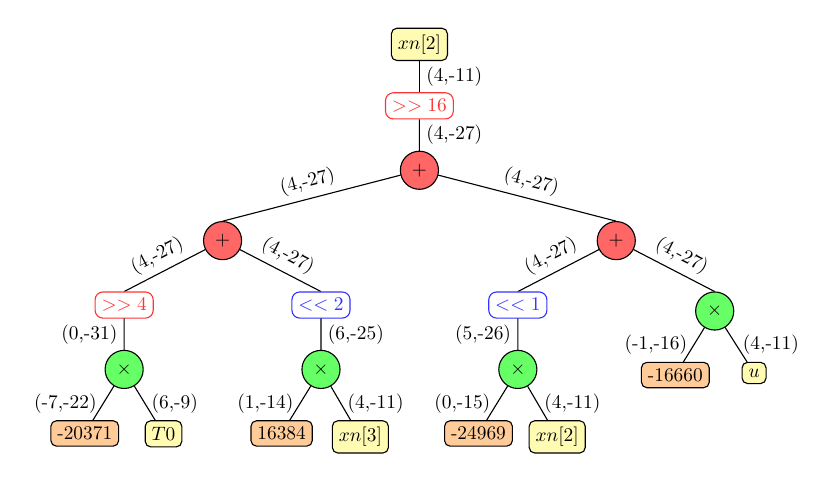
\begin{tikzpicture}[
     dec1/.style={rectangle, draw=red!80, rounded corners=1mm, fill=white,
        text centered, anchor=north, text=red!80, scale = 0.7},
    dec2/.style={rectangle, draw=blue!80, rounded corners=1mm, fill=white,
        text centered, anchor=north, text=blue!80, scale = 0.7},
    adder/.style={circle, draw, fill=red!60,
        text centered, anchor=north, text=black, scale = 0.7},
    mult/.style={circle, draw, fill=green!60,
        text centered, anchor=north, text=black, scale = 0.7},
     cst/.style={rectangle, rounded corners=0.7mm, draw, fill=orange!40,
        text centered, anchor=north, text=black, scale = 0.7},
     var/.style={rectangle, rounded corners=0.7mm, draw, fill=yellow!30,
        text centered, anchor=north, text=black, scale = 0.7},
     fpr/.style = {scale = 0.7},
    level distance=0.4cm, growth parent anchor=south
]
\node (Sortie) [var] {$xn[2]$}
child{[sibling distance=5.000000cm]
	node(DAdd_106) [dec1] {$>>16 $}
	child{
		node(Add_106) [adder] {$+$}
	child{[sibling distance=2.500000cm]
		node(Add_105) [adder] {$+$}
		child{[sibling distance=1cm]
			node(DMultT0 gamma  31) [dec1] {$>>4 $}
			child{
				node(MultT0 gamma  31) [mult] {$\times$}
				child{
					node(Cst2) [cst] {-20371}
				edge from parent node[fpr, left] {(-7,-22)}
				}
				child{
					node(Var2) [var] {$T0$}
				edge from parent node[fpr, right] {(6,-9)}
				}
				edge from parent node[fpr, left] {(0,-31)}
			}
			edge from parent node[fpr, left,sloped,above] {(4,-27)}
		}
		child{[sibling distance=1cm]
			node(DMultxn3 gamma  25) [dec2] {$<<2 $}
			child{
				node(Multxn3 gamma  25) [mult] {$\times$}
				child{
					node(Cst3) [cst] {16384}
				edge from parent node[fpr, left] {(1,-14)}
				}
				child{
					node(Var3) [var] {$xn[3]$}
				edge from parent node[fpr, right] {(4,-11)}
				}
				edge from parent node[fpr, right] {(6,-25)}
			}
			edge from parent node[fpr, right,sloped,above] {(4,-27)}
		}
		edge from parent node[fpr, left,sloped,above] {(4,-27)}
	}
	child{[sibling distance=2.500000cm]
		node(Add_73) [adder] {$+$}
		child{[sibling distance=1cm]
			node(DMultxn2 gamma  26) [dec2] {$<<1 $}
			child{
				node(Multxn2 gamma  26) [mult] {$\times$}
				child{
					node(Cst0) [cst] {-24969}
				edge from parent node[fpr, left] {(0,-15)}
				}
				child{
					node(Var0) [var] {$xn[2]$}
				edge from parent node[fpr, right] {(4,-11)}
				}
				edge from parent node[fpr, left] {(5,-26)}
			}
			edge from parent node[fpr, left,sloped,above] {(4,-27)}
		}
		child{[sibling distance=1cm]
			node(Multu gamma  27) [mult] {$\times$}
			child{
				node(Cst1) [cst] {-16660}
			edge from parent node[fpr, left] {(-1,-16)}
			}
			child{
				node(Var1) [var] {$u$}
			edge from parent node[fpr, right] {(4,-11)}
			}
			edge from parent node[fpr, right,sloped,above] {(4,-27)}
		}
		edge from parent node[fpr, right,sloped,above] {(4,-27)}
	}
		edge from parent node[fpr, right] {(4,-27)}	}
	edge from parent node[fpr, right] {(4,-11)}
}

;
        
\end{tikzpicture}
\end{center}
\end{document}